\subsection{Rimbalzi}

Guardando l'istogramma 2D delle misure in coincidenza, abbiamo notato dei comportamenti non attesi che abbiamo supposto e poi verificato essere dei fotoni che rimbalzano da un rivelatore all'altro.

La \autoref{scatter} mostra un tipico istogramma 2D
nella configurazione in cui 2 rivelatori sono posti uno di fronte all'altro alla stessa distanza da una sorgente di \na{}.

\begin{figure}[h]
\centering
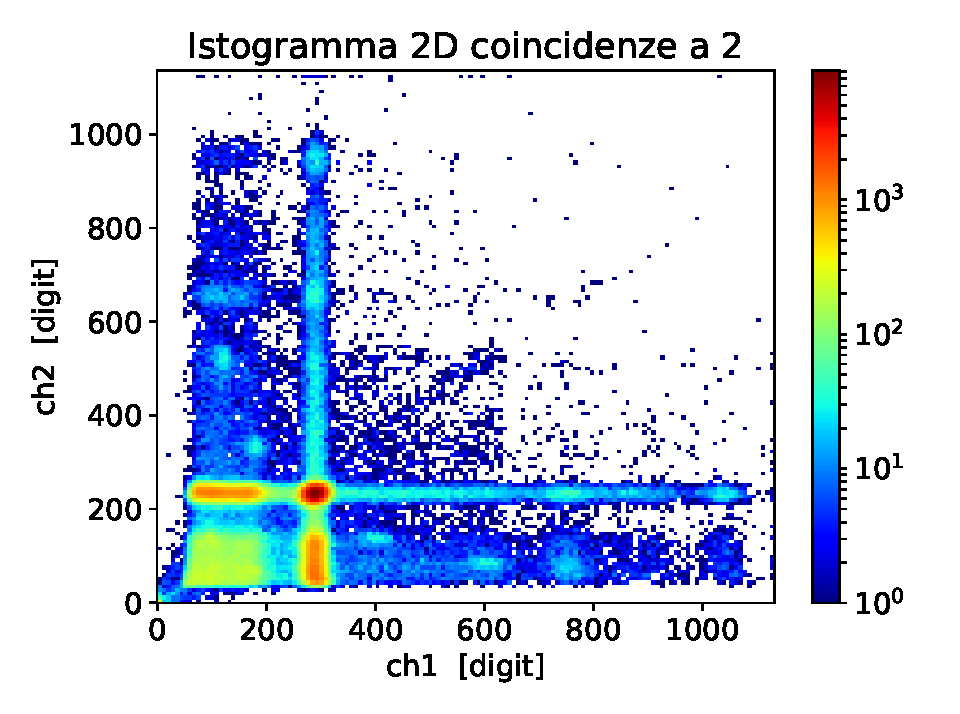
\includegraphics[width=\textwidth]{immagini/esempio}
\caption{Tipico istogramma 2D di una misura in coincidenza. La descrizione di questo grafico è presente nel testo.}
\label{scatter}
\end{figure}

\marginpar{Chiedere a Jack di fare il super grafico con istogrammi 1D e 2D se non si perde troppo tempo. Tra l'altro se non lo facciamo ci cazziano: ``Non avete inserito l'istogramma. Non si capisce niente.'' E non sarebbe male mettere una legenda sui picchi. }

Si vedono degli eccessi in alcuni punti del grafico che chiameremo in seguito \emph{strutture}. La più vistosa si manifesta quando entrambi i fotoni di annichilazione effettuano un processo fotoelettrico all'interno degli scintillatori. In basso a sinistra si nota invece la zona in cui entrambi hanno subito una diffusione Compton. Le bande arancioni intorno a questa zona rappresentano invece gli eventi in cui un fotone proveniente dall'annichilazione ha fatto fotoelettrico su un rivelatore e l'altro ha fatto Compton sull'altro.
La stessa cosa avviene con il fotone proveniente dal decadimento del neon, rappresentato dalle strutture nella parte centrale del grafico adiacente ai bordi della figura. La struttura più a destra (o più in alto) rappresenta l'arrivo simultaneo di un fotone di annichilazione insieme ad uno del neon. L'interpretazione degli eventi è analoga a quelli descritti precedentemente.
Le strutture non attese sono i due eccessi presenti nella zona in cui il fotone del neon e quello dell'annichilazione fanno entrambi scattering Compton. Queste strutture si manifestano a valori di energia coincidenti ai picchetti della spalla Compton.
\marginpar{``Picchetti della spalla Compton'' non è molto chiaro, ma ci penserò più tardi a come aggiustarli.}

Per verificare la nostra ipotesi abbiamo messo i rivelatori nella configurazione di Figura\autoref{spostati}, in modo da poterci aggiungere dei mattoni di piombo come in Figura\autoref{spostati2}. \marginpar{AGGIUSTARE}
L'istogramma 2D corrispondente si trova in Figura\autoref{spostato}: la struttura più popolata non è più data dalla rivelazione simultanea dell'annichilazione per effetto fotoelettrico, ma dalla somma degli eventi nelle bande che si incrociano.
In questa configurazione non si nota più uno degli eccessi inattesi nominati prima: quello ad energia minore.

\marginpar{Aggiungere il fatto che i picchi di rimbalzo sono in punti in cui le energie sommano a: $\beta$ (picchi nella zona sotto $\beta\beta$), $2\beta$ (picchi <<a energia minore>>), $\gamma$ (picchi più agli estremi).
Questo spiega anche perché quelli a energia minore scompaiono nella misura dei rimbalzi.}

Adesso sono diventate evidenti due strutture circolari nella zona in basso a sinistra del grafico: esse e l'ultimo tipo di struttura rimasta scompaiono completamente quando effettuiamo la misura nella configurazione mostrata in Figura\autoref{spostati2}, come mostrato in Figura\autoref{piombo}.

\begin{figure}[h]
\centering
\subfloat
{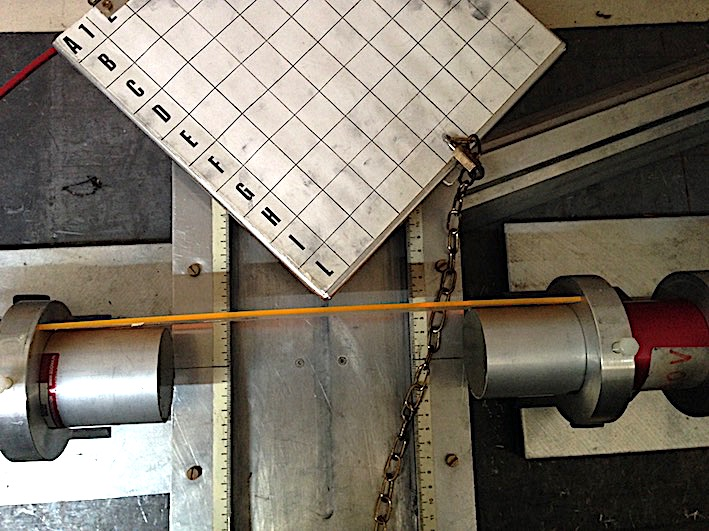
\includegraphics[width=0.49\textwidth]{immagini/alter}\label{spostati}}
\hfill
\subfloat
{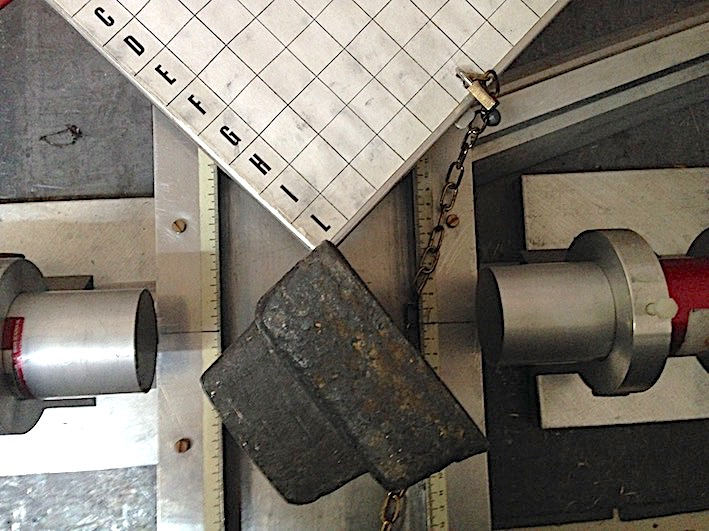
\includegraphics[width=0.49\textwidth]{immagini/spostati2}\label{spostati2}}
\caption{
A sinistra:
rivelatori posti uno di fronte all'altro senza schermatura.
La sorgente è nascosta nella casella L1 della scacchiera.
Il righello arancione serve per controllare che i due fotoni contrapposti di annichilazione
non possano raggiungere entrambi gli scintillatori.
A destra: aggiunta della schermatura di piombo per sopprimere i rimbalzi.}
\end{figure}

\begin{figure}[h]
\centering
\hspace{-2.5 cm}
\subfloat
{
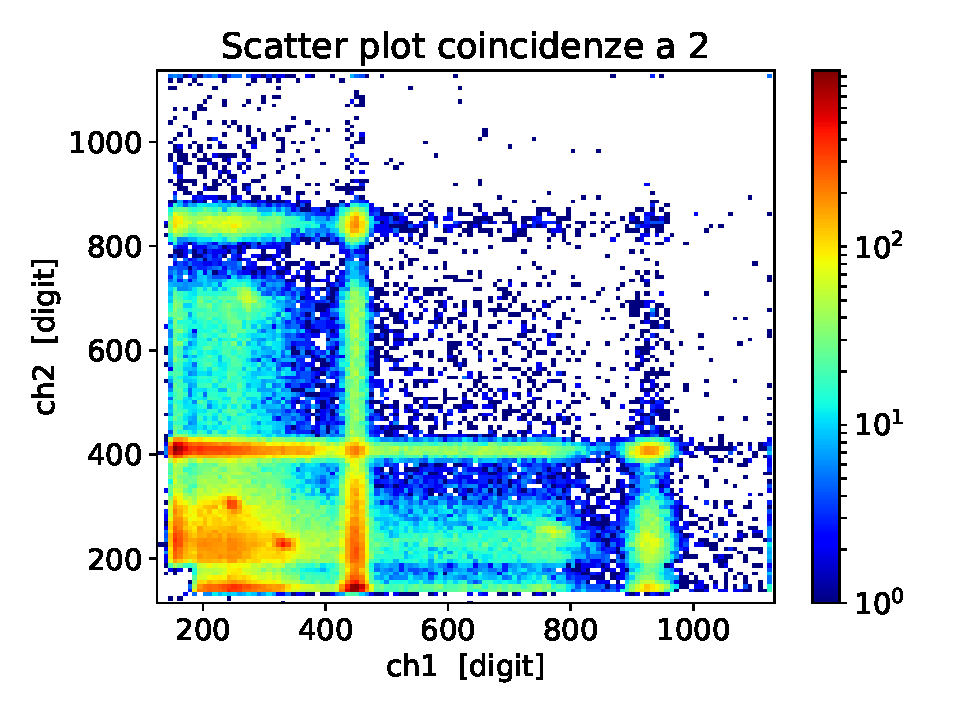
\includegraphics[width=21 em]{immagini/0518_rimbalzi}
\label{spostato}
}
\subfloat
{
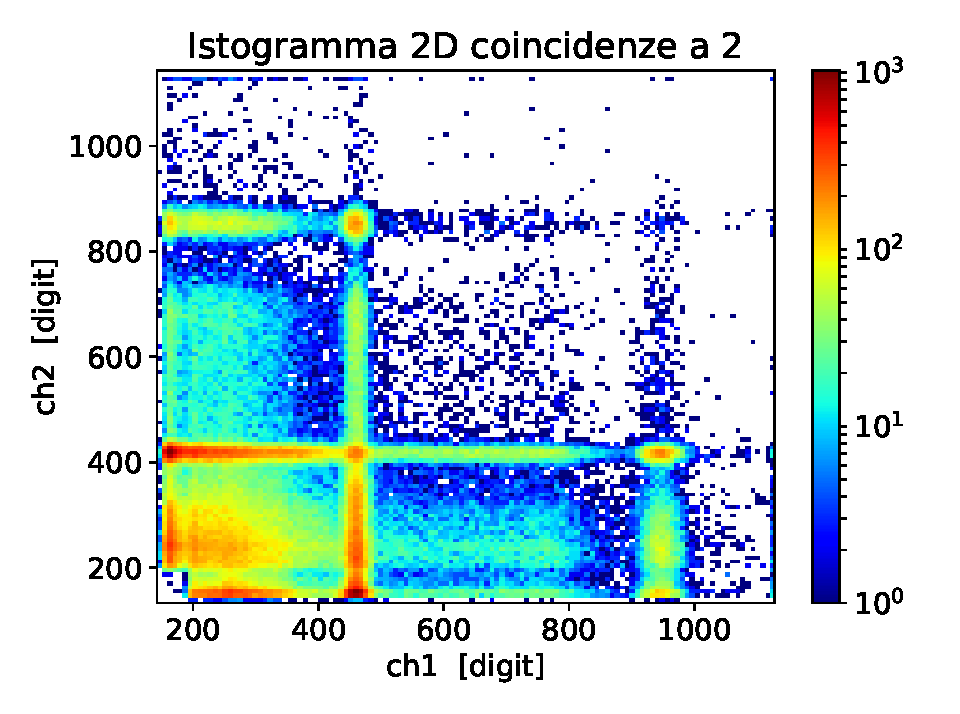
\includegraphics[width=21 em]{immagini/0518_piombo}
\label{piombo}
}
\caption{A sinistra: misura eseguita nella configurazione di Figura\autoref{spostati}. \\
A destra: misura eseguita nella configurazione di Figura\autoref{spostati2}.  \\
Le fasce densamente popolate adiacenti ai bordi della figura sono date dagli eventi in cui un rivelatore registra un evento mentre l'altro acquisisce uno zero.
Una descrizione più dettagliata di questi grafici è presente nel testo.}

\end{figure}

\subsubsection{Misura con un solo fotone}

Abbiamo effettuato la misura nella configurazione di \autoref{solo} sinistra e poi \autoref{solo} destra usando la sorgente di \cs{}: lo scopo della misura è evidenziare l'importanza dei rimbalzi tra scintillatori vicini.

\begin{figure}[h]
\centering
\subfloat
{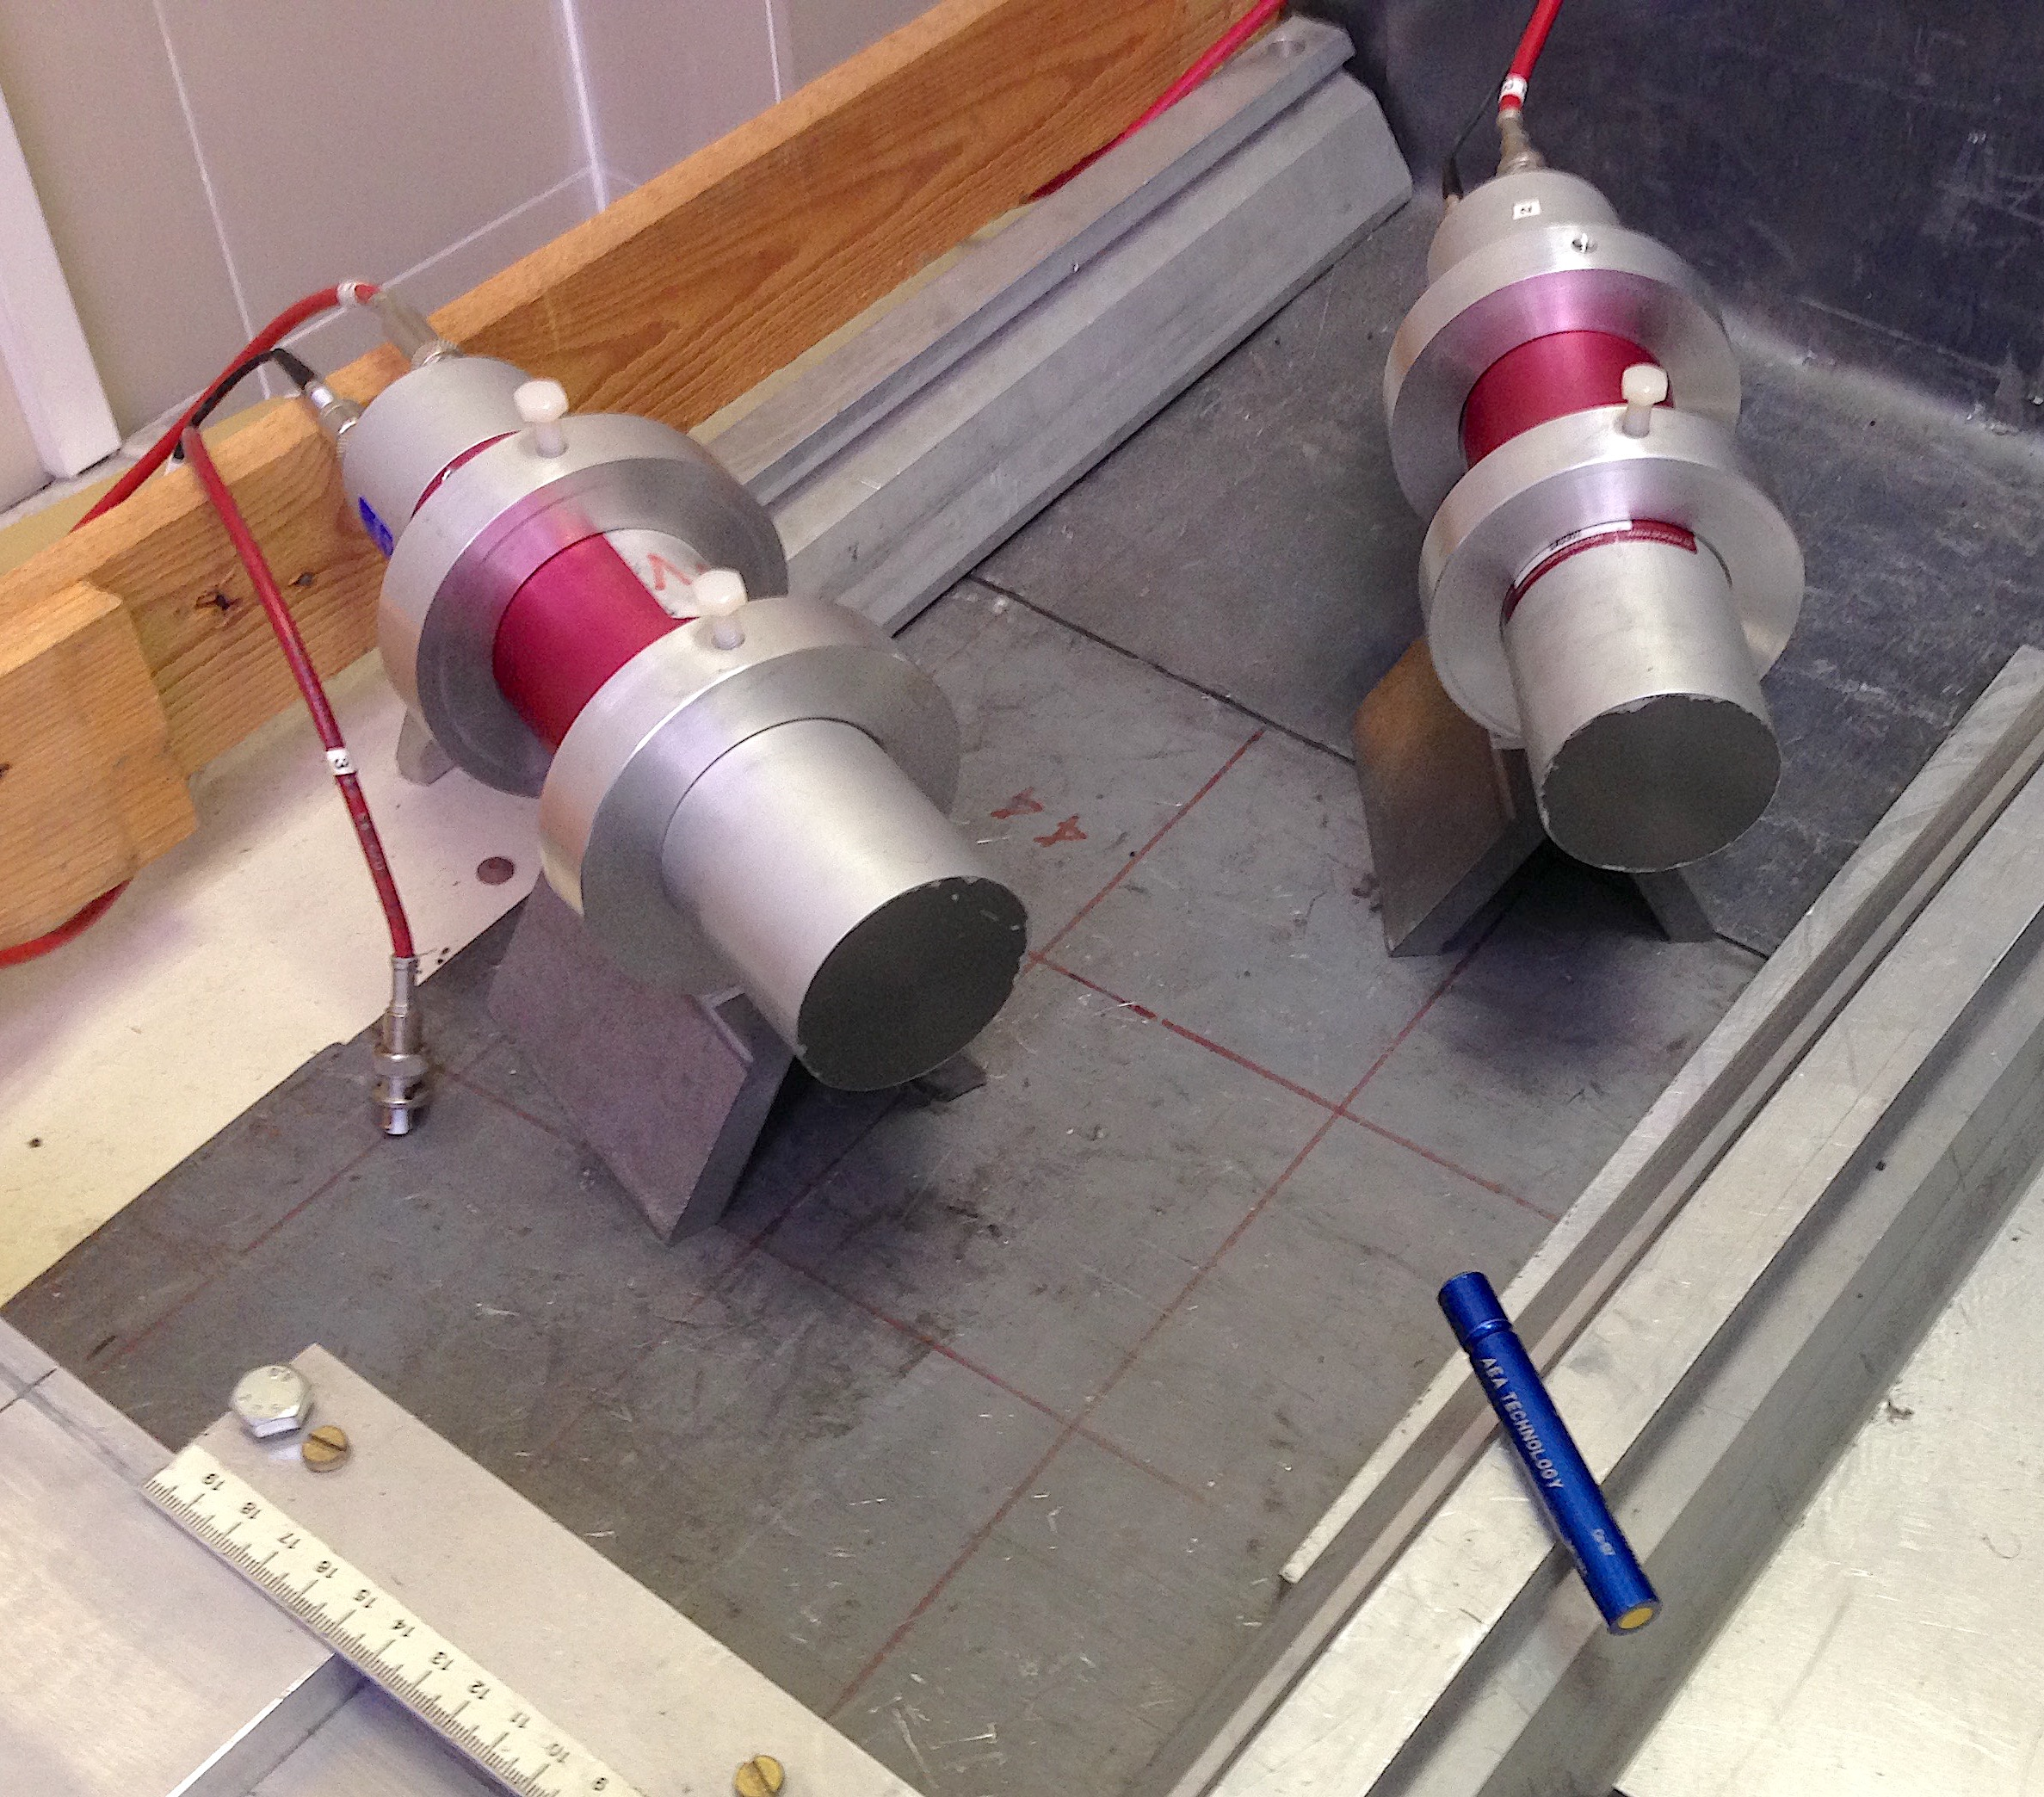
\includegraphics[width=0.49\textwidth]{immagini/rimb.jpg}}
\hfill
\subfloat
{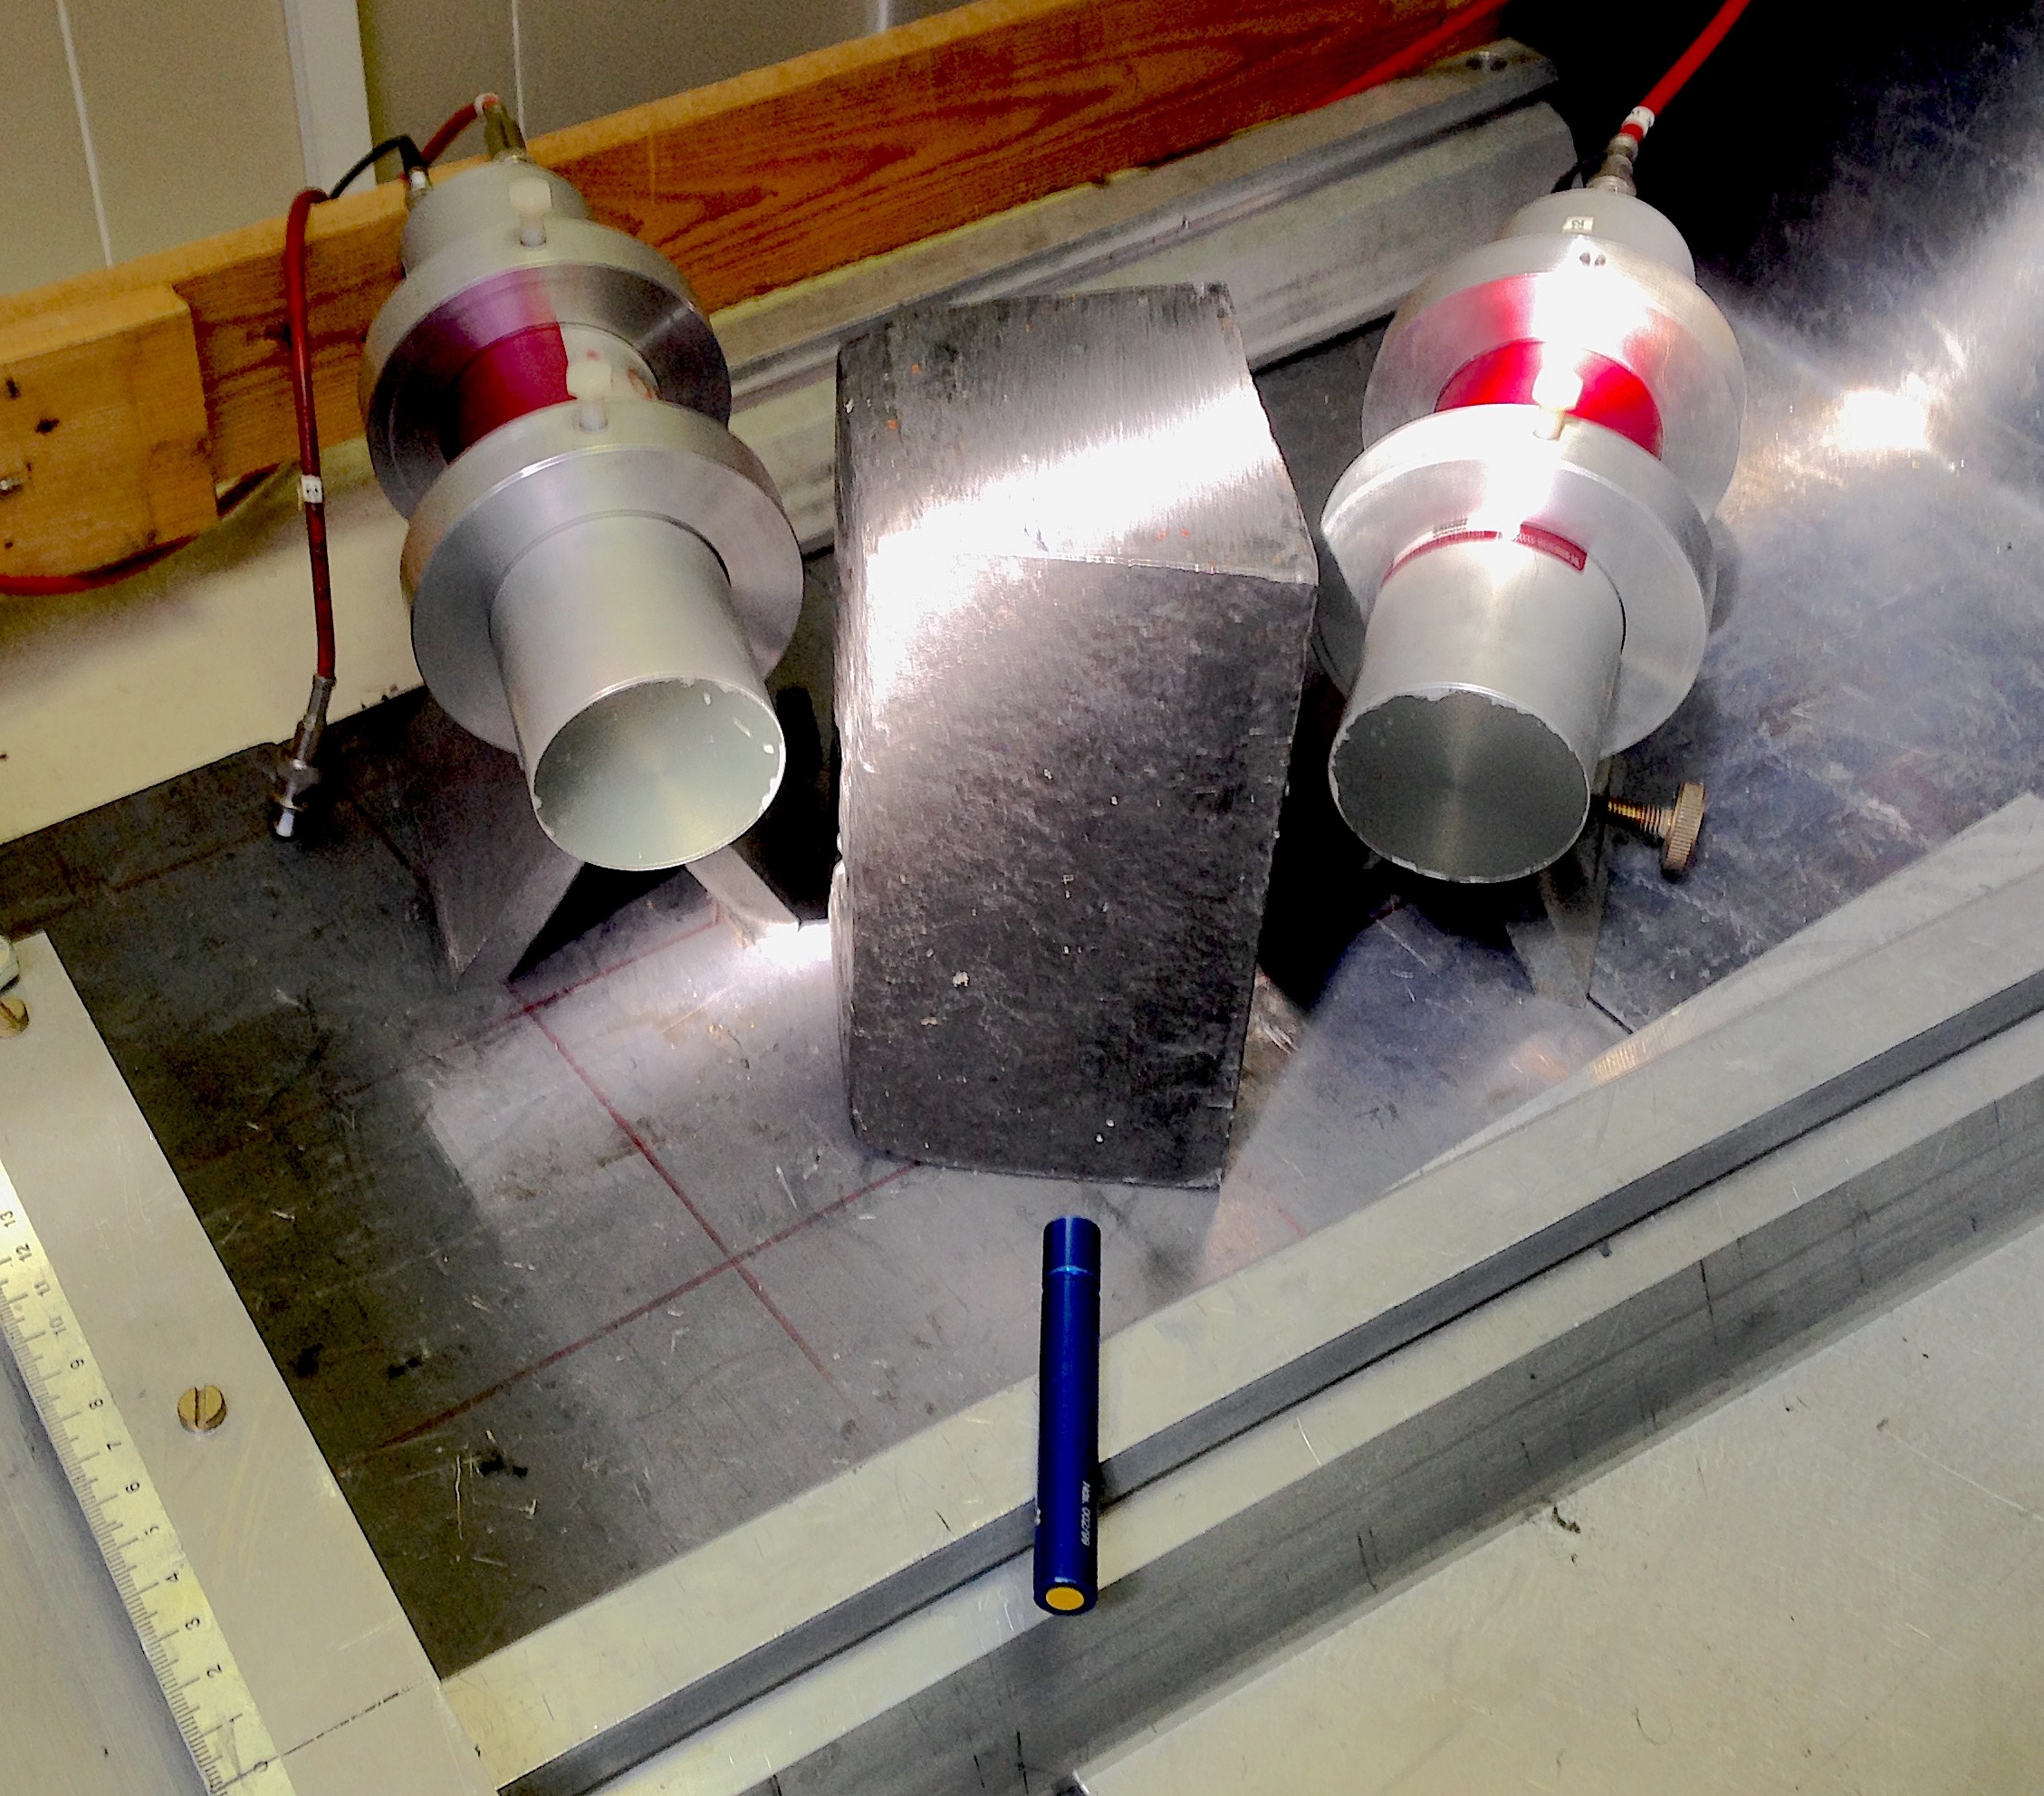
\includegraphics[width=0.49\textwidth]{immagini/norimb}}
\caption{\label{solo}
A sinistra:
configurazione usata per evidenziare la presenza di rimbalzi.
La sorgente è nel cilindretto blu.
A destra:
aggiunta del piombo che blocca i rimbalzi.}
\end{figure}

\begin{figure}[h]
\centering
% \subfloat
% {
% 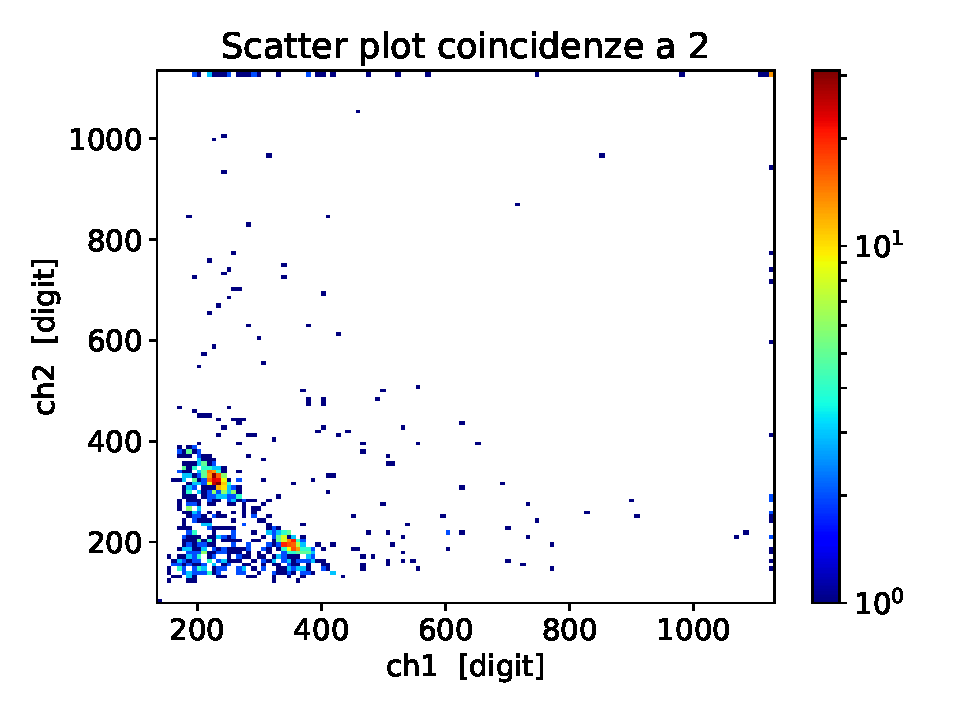
\includegraphics[width=18 em]{immagini/ce_ri}
% \label{ce}
% }
% \subfloat
% {
% 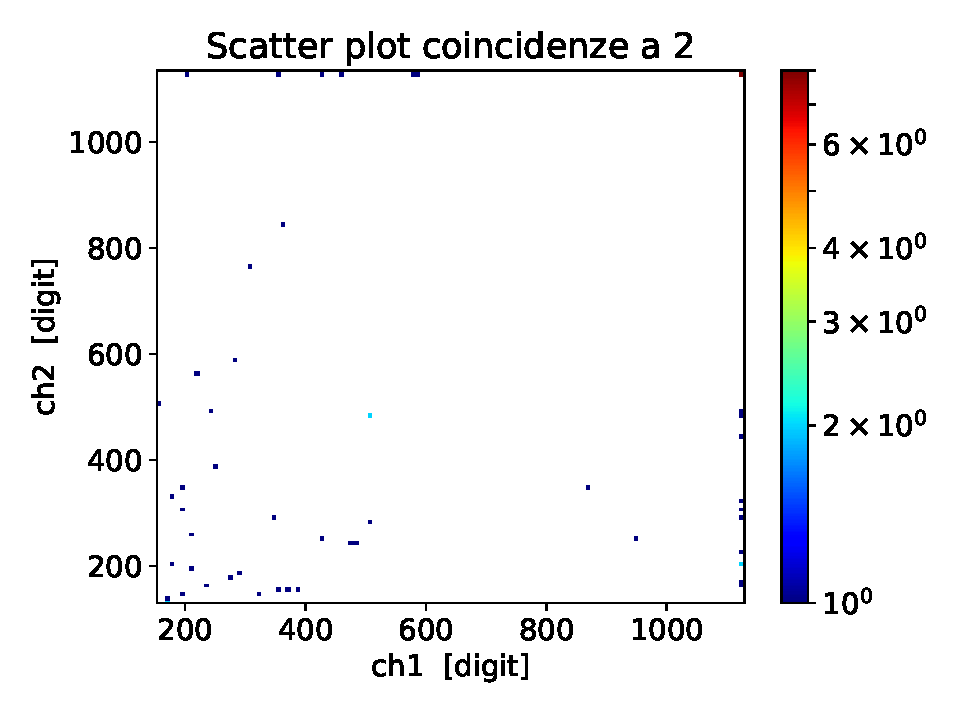
\includegraphics[width=18 em]{immagini/ce_pb}
% \label{no_ce}
% }
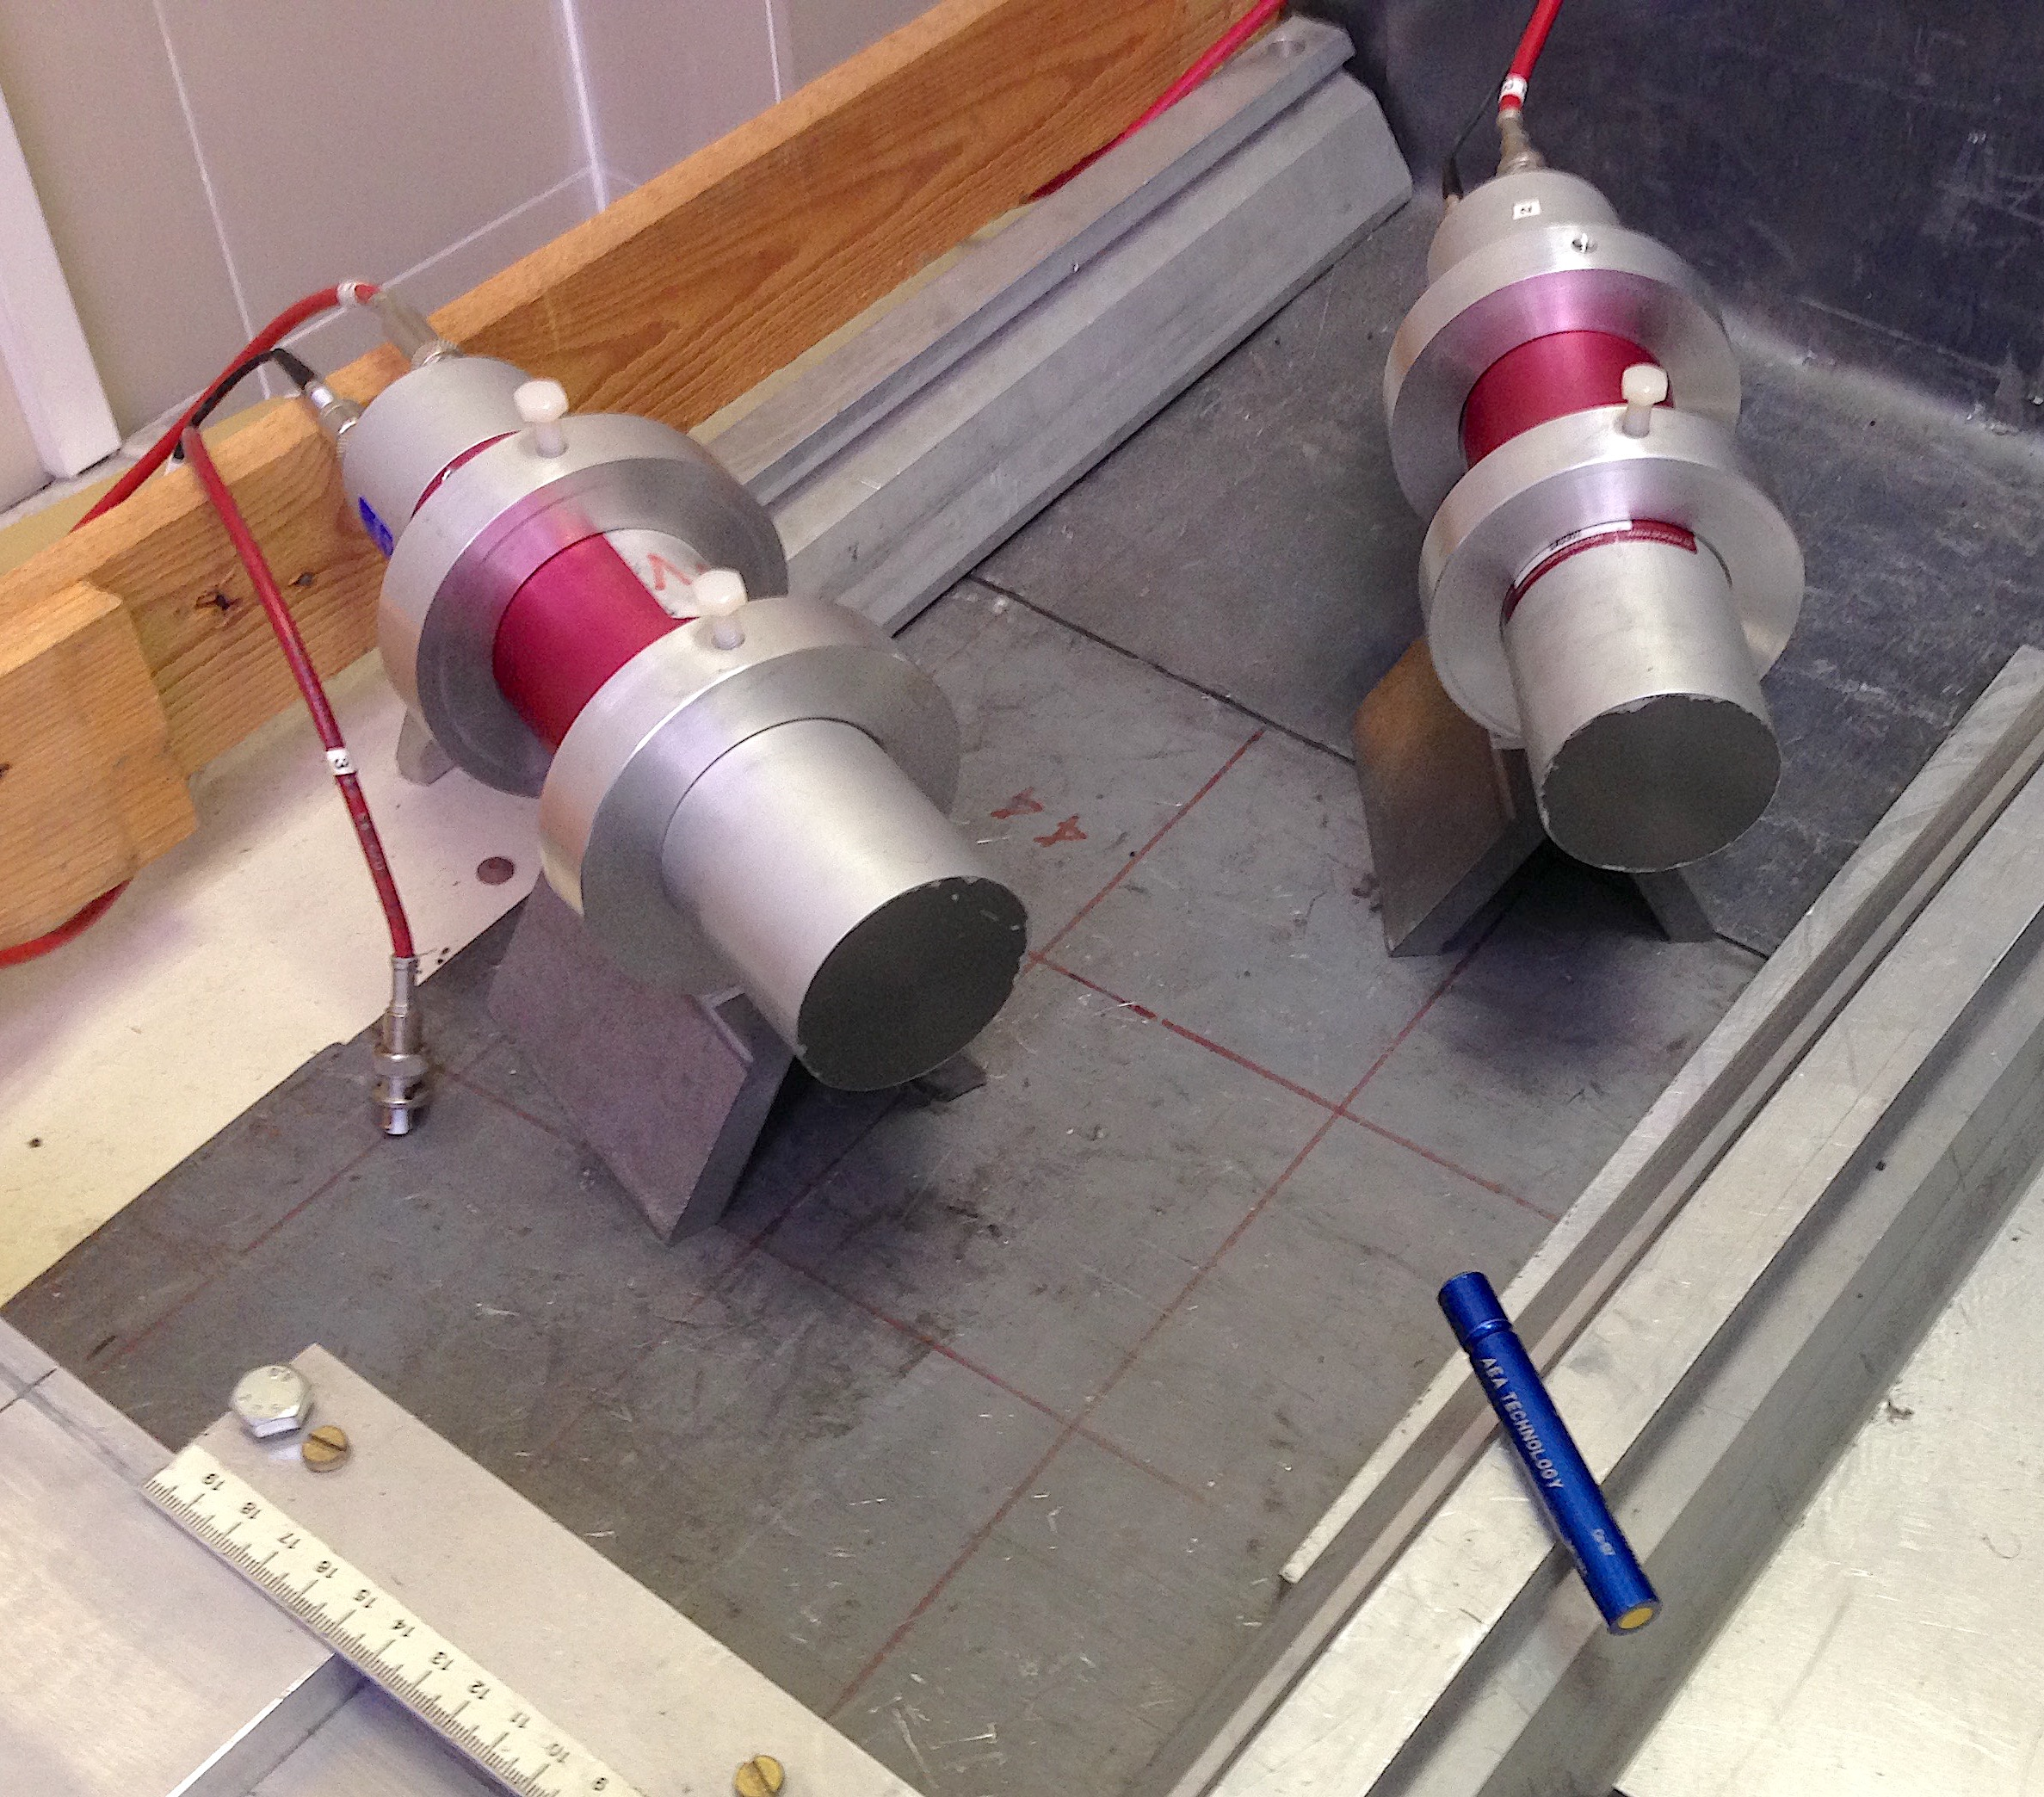
\includegraphics[width=\textwidth]{immagini/rimb}
\caption{\label{ce}
Spettro delle coincidenze tra i due scintillatori.
A sinistra: misura eseguita nella configurazione di \autoref{solo} sinistra.
A~destra: misura eseguita nella configurazione di \autoref{solo} destra.}
\end{figure}

L'istogramma 2D corrispondente alla \autoref{solo} sinistra è in \autoref{ce} sinistra: notiamo due accumuli proprio dove si trovavano in \autoref{spostato}. Anche questi scompaiono dopo aver aggiunto il piombo (\autoref{ce} destra). Gli eventi misurati non possono che essere coincidenze casuali.
\marginpar{Limare la fine della frase.
\\\emph{Non possono essere fotoni che passano il piombo? O che fanno doppio rimbalzo?}}

